% =============================================================================
%  CHAPTER 10: TikZ Graphics
% =============================================================================

\chapter{TikZ Graphics}

TikZ (``TikZ ist kein Zeichenprogramm'') is a powerful package for creating graphics directly in \latex{}.

\section{Basic Shapes}

\begin{figure}[H]
\centering
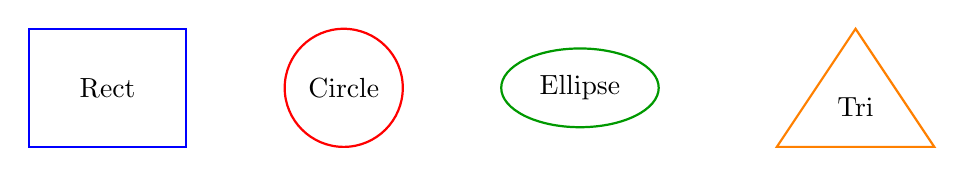
\begin{tikzpicture}
    % Rectangle
    \draw[thick, blue] (0,0) rectangle (2,1.5);
    \node at (1, 0.75) {Rect};

    % Circle
    \draw[thick, red] (4, 0.75) circle (0.75);
    \node at (4, 0.75) {Circle};

    % Ellipse
    \draw[thick, green!60!black] (7, 0.75) ellipse (1 and 0.5);
    \node at (7, 0.75) {Ellipse};

    % Triangle
    \draw[thick, orange] (9.5, 0) -- (11.5, 0) -- (10.5, 1.5) -- cycle;
    \node at (10.5, 0.5) {Tri};
\end{tikzpicture}
\caption{Basic shapes in TikZ}
\label{fig:tikzshapes}
\end{figure}

\begin{lstlisting}[language={[LaTeX]TeX}, caption=Basic shapes]
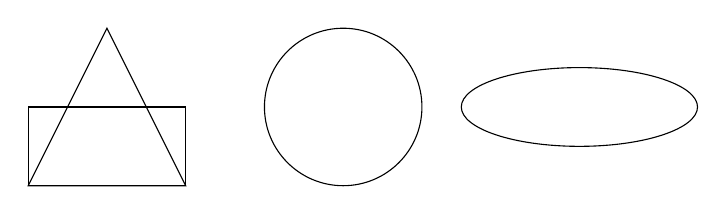
\begin{tikzpicture}
    \draw (0,0) rectangle (2,1);         % Rectangle
    \draw (4,1) circle (1);               % Circle
    \draw (7,1) ellipse (1.5 and 0.5);   % Ellipse
    \draw (0,0) -- (2,0) -- (1,2) -- cycle;  % Triangle
\end{tikzpicture}
\end{lstlisting}

% ------------------------------------------------------------------
\section{Lines and Paths}

\begin{figure}[H]
\centering
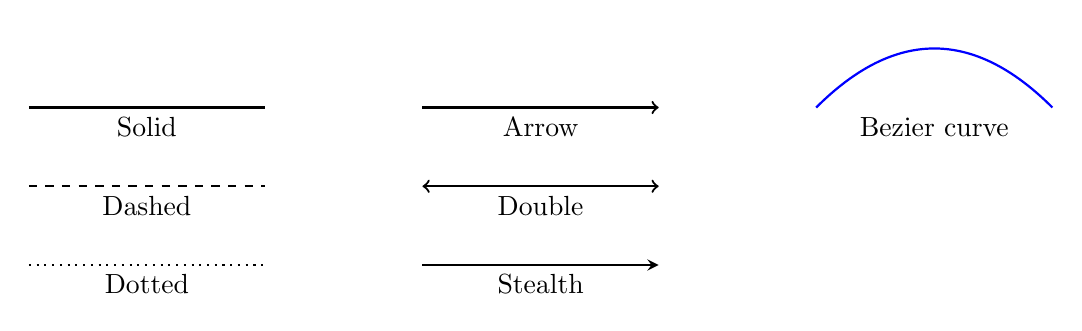
\begin{tikzpicture}
    % Solid line
    \draw[thick] (0,0) -- (3,0);
    \node[below] at (1.5,0) {Solid};

    % Dashed line
    \draw[thick, dashed] (0,-1) -- (3,-1);
    \node[below] at (1.5,-1) {Dashed};

    % Dotted line
    \draw[thick, dotted] (0,-2) -- (3,-2);
    \node[below] at (1.5,-2) {Dotted};

    % Arrow
    \draw[thick, ->] (5,0) -- (8,0);
    \node[below] at (6.5,0) {Arrow};

    % Double arrow
    \draw[thick, <->] (5,-1) -- (8,-1);
    \node[below] at (6.5,-1) {Double};

    % Stealth arrow
    \draw[thick, >=stealth, ->] (5,-2) -- (8,-2);
    \node[below] at (6.5,-2) {Stealth};

    % Curved path
    \draw[thick, blue] (10,0) .. controls (11,1) and (12,1) .. (13,0);
    \node[below] at (11.5,0) {Bezier curve};
\end{tikzpicture}
\caption{Lines and paths in TikZ}
\label{fig:tikzlines}
\end{figure}

% ------------------------------------------------------------------
\section{Filling and Colors}

\begin{figure}[H]
\centering
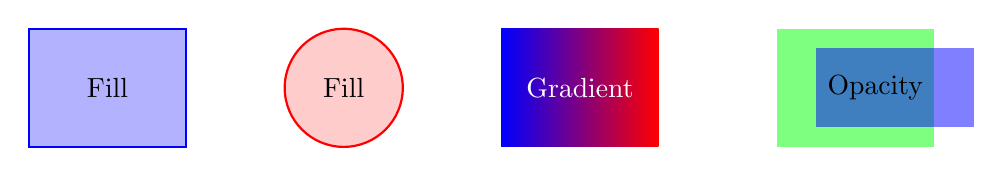
\begin{tikzpicture}
    % Filled shapes
    \fill[blue!30] (0,0) rectangle (2,1.5);
    \draw[blue, thick] (0,0) rectangle (2,1.5);
    \node at (1, 0.75) {Fill};

    \filldraw[fill=red!20, draw=red, thick] (4, 0.75) circle (0.75);
    \node at (4, 0.75) {Fill};

    % Gradient
    \shade[left color=blue, right color=red] (6,0) rectangle (8,1.5);
    \node[white] at (7, 0.75) {Gradient};

    % Opacity
    \fill[green, opacity=0.5] (9.5,0) rectangle (11.5,1.5);
    \fill[blue, opacity=0.5] (10,0.25) rectangle (12,1.25);
    \node at (10.75, 0.75) {Opacity};
\end{tikzpicture}
\caption{Filling and colors in TikZ}
\label{fig:tikzfill}
\end{figure}

% ------------------------------------------------------------------
\section{Nodes and Labels}

\begin{figure}[H]
\centering
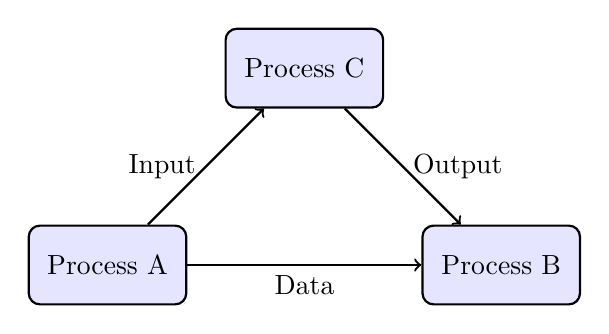
\begin{tikzpicture}[
    box/.style={rectangle, draw, thick, minimum width=2cm, minimum height=1cm,
                fill=blue!10, rounded corners, align=center},
    circle node/.style={circle, draw, thick, fill=red!10, minimum size=1cm}
]
    \node[box] (a) at (0,0) {Process A};
    \node[box] (b) at (5,0) {Process B};
    \node[box] (c) at (2.5,2.5) {Process C};

    \draw[->, thick] (a) -- (b) node[midway, below] {Data};
    \draw[->, thick] (a) -- (c) node[midway, left] {Input};
    \draw[->, thick] (c) -- (b) node[midway, right] {Output};
\end{tikzpicture}
\caption{Nodes and connections in TikZ}
\label{fig:tikznodes}
\end{figure}

\begin{lstlisting}[language={[LaTeX]TeX}, caption=Nodes and edges]
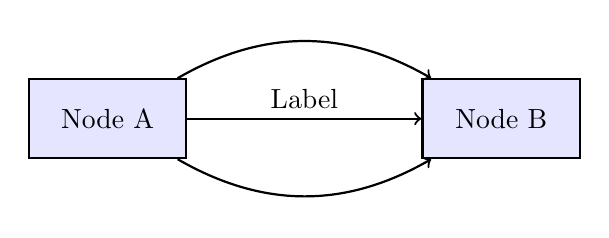
\begin{tikzpicture}[
    box/.style={rectangle, draw, thick, fill=blue!10,
                minimum width=2cm, minimum height=1cm}
]
    \node[box] (a) at (0,0) {Node A};
    \node[box] (b) at (5,0) {Node B};

    \draw[->, thick] (a) -- (b) node[midway, above] {Label};
    \draw[->, thick, bend left=30] (a) to (b);
    \draw[->, thick, bend right=30] (a) to[bend right] (b);
\end{tikzpicture}
\end{lstlisting}

% ------------------------------------------------------------------
\section{Flowchart}

% Uses the shapes.geometric library (for diamond) and positioning library
% (for below=of syntax). Both loaded in main.tex preamble.

\begin{figure}[H]
\centering
\begin{tikzpicture}[
    % Define reusable styles — these are just key-value defaults
    startstop/.style={rectangle, rounded corners, minimum width=3cm, minimum height=0.8cm,
                      text centered, draw=black, fill=red!20},
    process/.style={rectangle, minimum width=3cm, minimum height=0.8cm,
                    text centered, draw=black, fill=blue!15},
    decision/.style={diamond, aspect=2, minimum width=2.5cm,
                     text centered, draw=black, fill=green!15},
    arrow/.style={thick, -Stealth}   % -Stealth uses arrows.meta library
]
    \node (start)    [startstop]                    {Start};
    \node (input)    [process,  below=1cm of start] {Read Input};
    \node (decision) [decision, below=1cm of input] {Valid?};
    \node (process1) [process,  below=1cm of decision] {Process Data};
    \node (output)   [process,  right=3cm of decision] {Show Error};
    \node (stop)     [startstop, below=1cm of process1] {Stop};

    \draw [arrow] (start)    -- (input);
    \draw [arrow] (input)    -- (decision);
    \draw [arrow] (decision) -- node[left]  {Yes} (process1);
    \draw [arrow] (decision) -- node[above] {No}  (output);
    \draw [arrow] (output)   |- (input);
    \draw [arrow] (process1) -- (stop);
\end{tikzpicture}
\caption{Flowchart using TikZ (requires \texttt{shapes.geometric} and \texttt{positioning} libraries)}
\label{fig:flowchart}
\end{figure}

% ------------------------------------------------------------------
\section{Plots with pgfplots}

\begin{figure}[H]
\centering
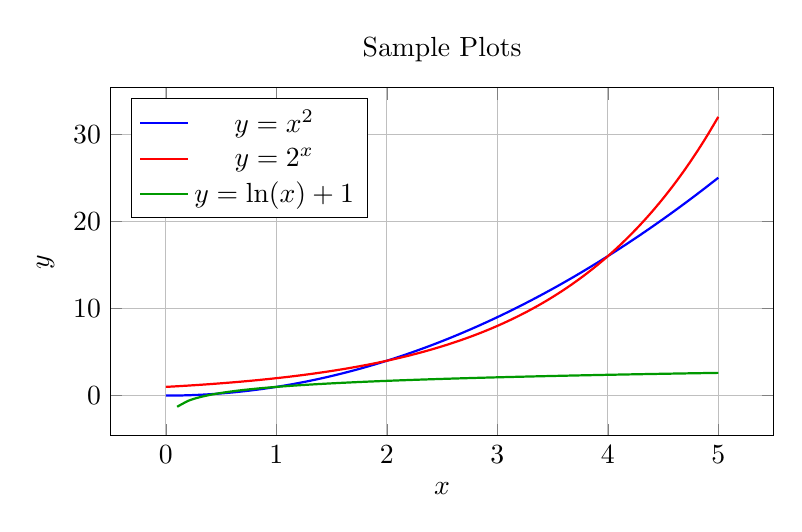
\begin{tikzpicture}
    \begin{axis}[
        xlabel={$x$},
        ylabel={$y$},
        title={Sample Plots},
        legend pos=north west,
        grid=major,
        width=10cm,
        height=6cm,
    ]
        \addplot[blue, thick, smooth, domain=0:5, samples=50] {x^2};
        \addlegendentry{$y = x^2$}

        \addplot[red, thick, smooth, domain=0:5, samples=50] {2^x};
        \addlegendentry{$y = 2^x$}

        \addplot[green!60!black, thick, smooth, domain=0:5, samples=50] {ln(x)+1};
        \addlegendentry{$y = \ln(x) + 1$}
    \end{axis}
\end{tikzpicture}
\caption{Function plots using pgfplots}
\label{fig:pgfplots}
\end{figure}

\begin{lstlisting}[language={[LaTeX]TeX}, caption=pgfplots example]
\usepackage{pgfplots}
\pgfplotsset{compat=1.18}

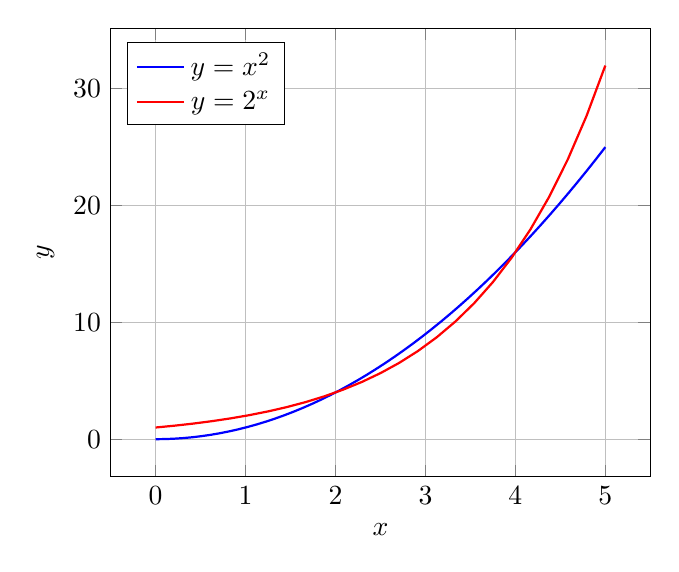
\begin{tikzpicture}
    \begin{axis}[
        xlabel={$x$}, ylabel={$y$},
        legend pos=north west,
        grid=major,
    ]
        \addplot[blue, thick, domain=0:5, samples=50] {x^2};
        \addlegendentry{$y = x^2$}

        \addplot[red, thick, domain=0:5] {2^x};
        \addlegendentry{$y = 2^x$}
    \end{axis}
\end{tikzpicture}
\end{lstlisting}

% ------------------------------------------------------------------
\section{Bar Chart}

\begin{figure}[H]
\centering
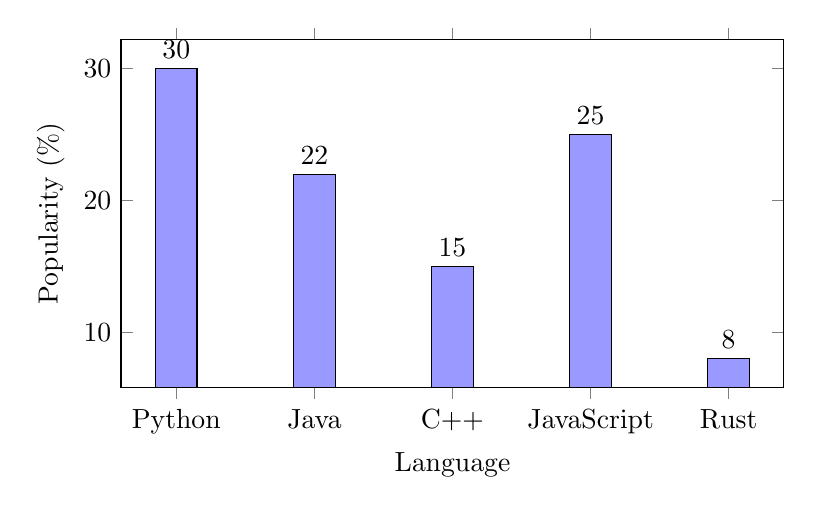
\begin{tikzpicture}
    \begin{axis}[
        ybar,
        xlabel={Language},
        ylabel={Popularity (\%)},
        symbolic x coords={Python, Java, C++, JavaScript, Rust},
        xtick=data,
        nodes near coords,
        nodes near coords align={vertical},
        width=10cm,
        height=6cm,
        bar width=15pt,
    ]
        \addplot[fill=blue!40] coordinates {
            (Python, 30) (Java, 22) (C++, 15) (JavaScript, 25) (Rust, 8)
        };
    \end{axis}
\end{tikzpicture}
\caption{Bar chart using pgfplots}
\label{fig:barchart}
\end{figure}

% ------------------------------------------------------------------
\section{TikZ Styles}

\begin{lstlisting}[language={[LaTeX]TeX}, caption=TikZ styles]
% Define reusable styles:
\tikzset{
    mybox/.style={
        rectangle, draw, thick,
        fill=blue!10,
        minimum width=2cm,
        minimum height=1cm,
        rounded corners=3pt,
        font=\sffamily
    },
    myarrow/.style={
        ->, >=stealth, thick, shorten >=1pt
    },
}

% Use them:
\node[mybox] (a) at (0,0) {Styled};
\node[mybox, fill=red!10] (b) at (3,0) {Override};
\draw[myarrow] (a) -- (b);
\end{lstlisting}
